% CREATED BY DAVID FRISK, 2016
\chapter{Results}
\label{ch:results}

First the purpose of the paper is repeated to motivate the results obtained below. The main purpose of this paper is to investigate if  and how the VAHSS construction \ref{alg:VAHSS-HSS} can be extended with a range proof to ensure honest clients. Beside this main purpose the aim is also to provide an implementation of such a combined construction and to compare different range proofs and their compatibility to VAHSS. The results for there three questions will be given below in three sub sections. 

\section{Combining}
The main result of this paper is that it is possible to combine a VAHSS construction as described in section \ref{sec:VAHSS} with a range proof to reduce the potential impact of malicious clients. Using range proofs (or set membership proofs) that assumes a Pedersen commitment the combining with the VAHSS construction becomes almost parallel in the sence that the VAHSS and range proof (or set membership proof) are run almost independent of each other. It was also found that the combination could be done without specifying the details about the range proof, hence any range proof that assumes a Pedersen commitment can be used, which leads to a highly flexible combination.  
%Note that although the construction does not specify which range proof that is used the implementation does due o the choice of group in the set up, the signature-based range proofs and set membership proof uses pairing friendly elliptic curve groups in the implementation which is not the case for Bulletproofs.

The main factor determining the suitability of different range proofs is their runtime and their possibility to be aggregated, since all can be combined using the same approach to the VAHSS construction. The two range proofs studied are Bulletproofs and signature-based range proofs and the runtime comparison between them showed that Bulletproofs were significantly faster, hence more suitable for using in server and client verifiable AHSS presented in Construction \ref{alg:VAHSS-HSS-RP}. 

\section{Runtime}

\begin{figure}[]
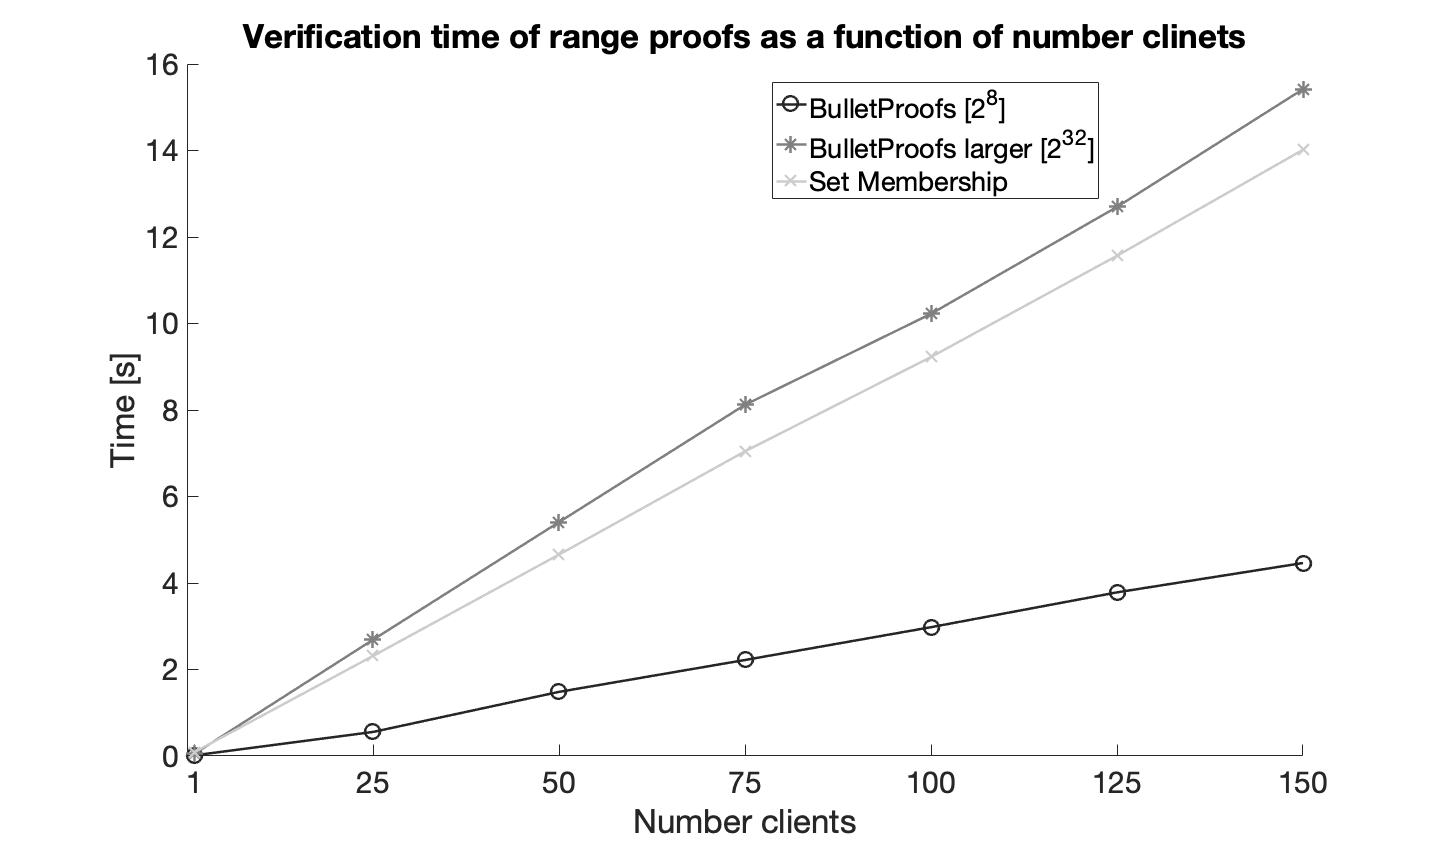
\includegraphics[width=\linewidth]{./figure/verification_nrClients.png}
\end{figure}


\begin{table}
\label{tab:BenchBP}
\caption{Timing in seconds for server and client verifiable-AHSS. Verfication of clients is done by usingBulletProofs}
\centering
\begin{tabular}{*{5}{c}}
\hline
    										&  \textbf{Executer}   & \multicolumn{3}{c}{\textbf{Time}}   		\\ 
    										& 								& Bullet proof  & signature based & Set membership \\	\hline
  GenerateShares 				&  client  					&   95 [$\mu$s]			 &96[$\mu$s]  &98 [$\mu$s]												\\ \hline 
  GenerateRangeProof  		&  clients  					&   53 [ms]				& 	241 [ms]	&66 [ms]			\\ \hline 
  PartialEval  						&  server  					&   78	[$\mu$s]				&72[$\mu$s]	 		&	71	 [$\mu$s]							\\ \hline 
  PartialProof 					&  server 					&   273[$\mu$s]						& 5249 [$\mu$s]			& 5255 [$\mu$s]				\\ \hline 
  FinalEval  						&  x  							&   689 [ns]						&655  [ns]				&			699  [ns]												\\ \hline 
  FinalProof  						&  x 							&   50	[$\mu$s]			&  114 [$\mu$s]	&				115 [$\mu$s]									\\ \hline 
  VerifyRP							&  x 							&   2979[ms]					&  &					9288 [ms]							\\ \hline 
  VerifyServers					&  x 							&   1672 [$\mu$s]					&		7990 [ms] 	&		7947 [$\mu$s]					\\ \hline 
\end{tabular}
 \end{table}